\chapterimage{finance.pdf}
\chapterimagecaption{\textit{At the Roulette Table in Monte Carlo} (1892) by Edvard Munch}

\chapter{Financial Information} \index{Finances}


    \section{Travel Guidelines} \index{Travel}
    When travelling on behalf of McGill there are four main things to arrange, depending on your specific circumstances: \textbf{Travel insurance, accommodation, transport, food, and visas}.    \href{https://www.mcgill.ca/financialservices/policies/reimburse/procedures}{\textbf{Read through this website first before proceeding.}}

     The aim of this section is to give a brief outline of the process as well as provide some information on grants and awards to fund your travel.


  \subsection{Travel Insurance} \index{Travel! Insurance}
    Travel insurance is essential so that you're covered for any emergency medical expenses abroad. The insurance is provided through PGSS or McGill at no additional cost.
    
    \begin{itemize}
    \item Canadian Citizens (anyone that accesses PGSS Health plan):\\
    Coverage provided by PGSS, see this \href{https://studentcare.ca/rte/en/McGilluniversitygraduatestudentspgss\_Travel\_TravelCoverage}{site}.\vspace{5pt}

    \item International Students:\\
    Coverage provided through \href{https://www.mcgill.ca/internationalstudents/health/benefits/going-abroad}{extension} of Blue Cross International Health Insurance (up to 4 weeks).
    \end{itemize}

    \subsection{Accomodation} \index{Travel! Accomodation}
    \begin{itemize}
    \item Before booking anywhere to stay, first determine if your conference/event provides any funding for accommodation (many do!). If this is the case, there will likely be a per night price limit up to which they will reimburse, as well as a restriction on how many nights before/after the scheduled programming they will support. For example, if the conference runs Monday to Friday, they most likely will fund Sunday night to Friday night inclusive.
    \item If the event will not provide any lodging support, speak with your supervisor to determine if they will support your stay. Most groups in the physics department will fund their student’s accommodation.
    \item If your accommodation is covered (either by your supervisor’s grant funds or by the conference hosts), it will likely be in the form of a reimbursement after the event. It is therefore recommended to look for accommodation that only requires you to pay the full amount nearer/upon check in, so that the money is not tied up for months on end.
    \item To be reimbursed with your supervisor’s grant funds, you should follow the guide below on reimbursements (section \hyperref[section:reimbursement]{\textcolor{purble}{\ref*{section:reimbursement}}}).
    \item The process to obtain reimbursement from the event organizers will vary depending on the host institution. However, most events will have dedicated in house organization/admin staff to assist with this process.
    \item Many conferences will provide hotel recommendations upon registration, so be sure to look out for these!\\

    \end{itemize}


    \subsection{Transport} \index{Travel! Transport}

    \noindent If you need to take a flight, there are two main ways to approach booking and paying for it:
    \begin{enumerate}
        \item Direct billing of your supervisor’s grant fund
        \item You pay (and then are possibly reimbursed)
    \end{enumerate}

    \noindent The first method is recommended, so you are not out of pocket for the months leading up to the event. If you're going to take a train/coach/anything else, this option is not available, so you must book with your own money and then seek reimbursement (see section \hyperref[section:reimbursement]{\textcolor{purble}{\ref*{section:reimbursement}}}).\\

    \subsection*{Guide for direct billing method}  
    (Read in it’s entirety before proceeding)\\

    \begin{itemize}[leftmargin=10pt]
        \item Go to \url{https://www.mcgill.ca/travelservices/transport/tmc} and click ‘Create New Profile’. Enter your details, then wait for the account to be approved by admin staff. Then log in by clicking ‘Access Existing Profile’.
        \begin{figure}[H]
            \centering
            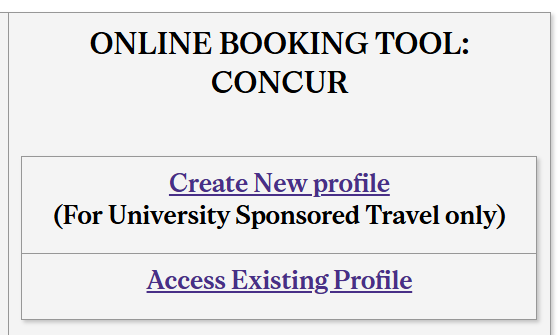
\includegraphics[width=0.4\columnwidth]{Pictures/CreateAccount.png}
        \end{figure}

        \item Navigate to the flight tab, and read the provided instructions for an overview of the process. Note that the Workday step at the end is only available from September to April. Over the summer, this step can be completed by submitting a ticket to the Finance Service Desk (\url{https://hrservicedesk.mcgill.ca/servicedesk/customer/portal/12}), under the category ‘WE-Airfare/Rail (Spend Authorization’. 

        \begin{figure}[H]
            \centering
            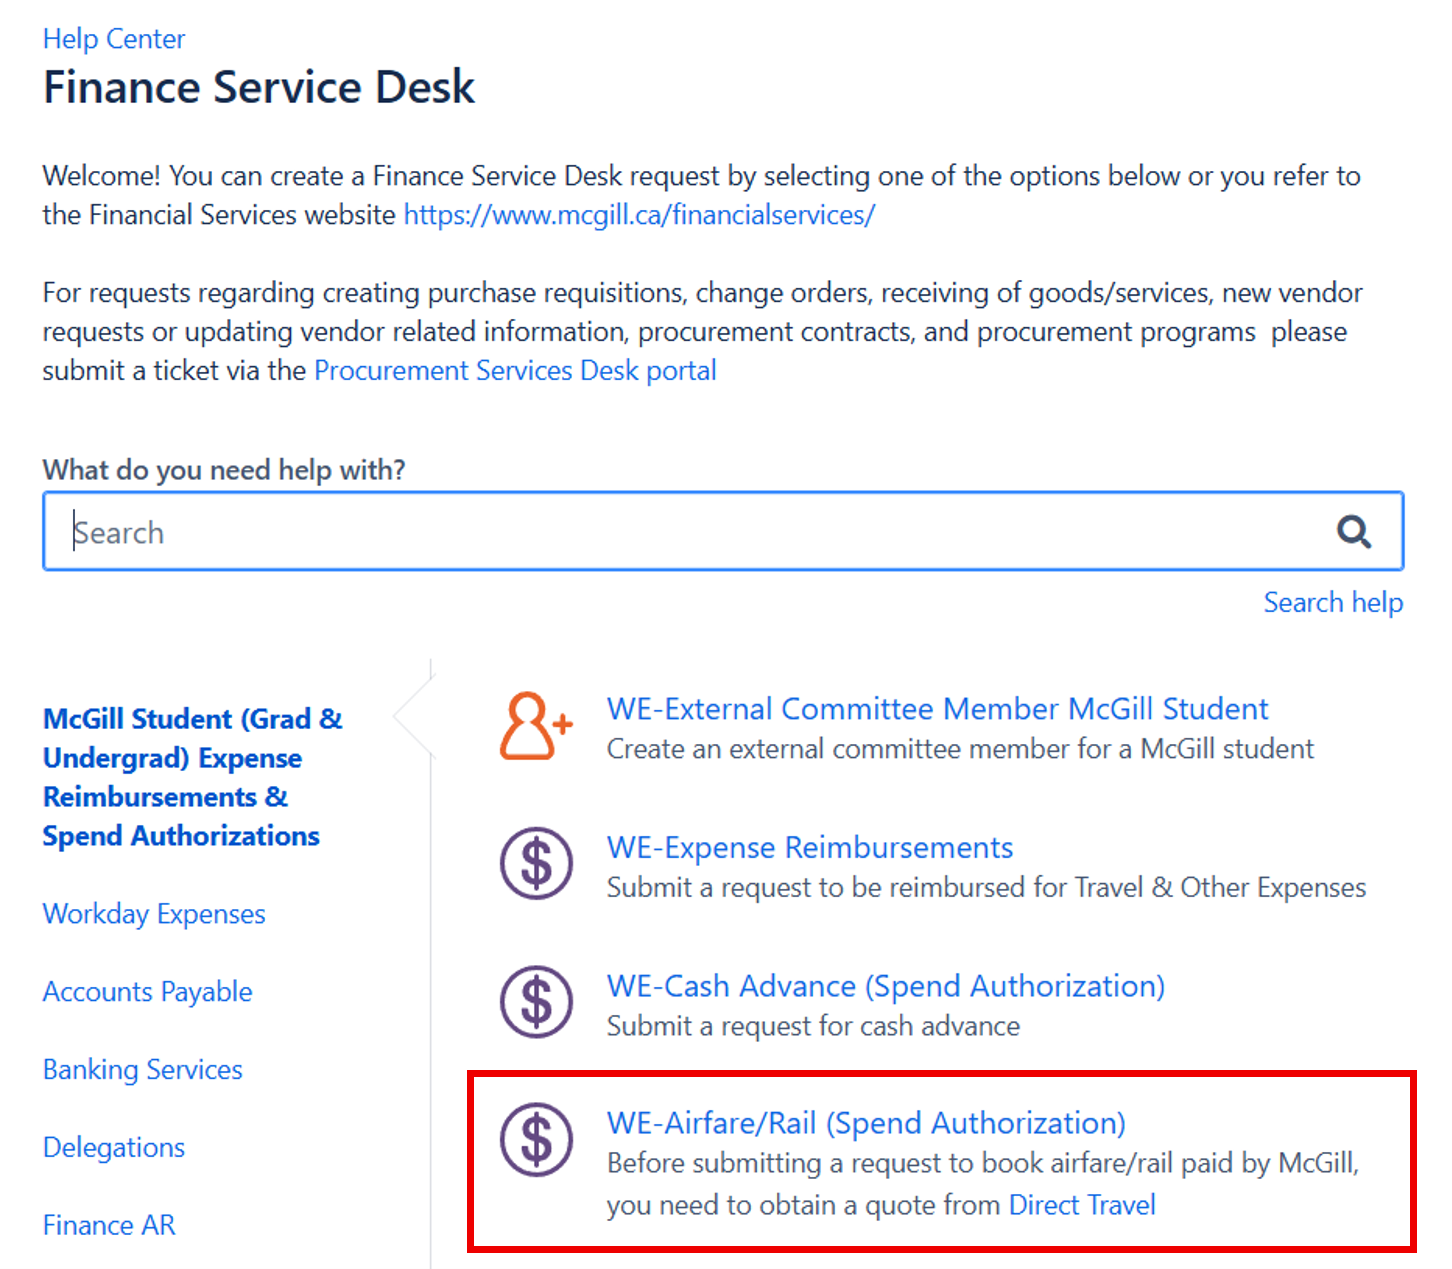
\includegraphics[width=0.65\columnwidth]{Pictures/SpendAuth.png}
        \end{figure}

        \item \textbf{\color{ocre}Important:} This approval can only be processed during regular business hours (Mon - Fri 08:30 - 17:00). The flight can only be held for 24 hours, so it is recommended that you only proceed from here between Monday morning and Friday morning, and account for any public holidays.\\

        \item Use the search tool to find appropriate flights. Find the cheapest flights that don’t have a ridiculous layover, or your supervisor may refuse to pay (i.e. no business class). You should take screenshot proof that you have selected a low cost flight relative to equivalents. Be sure to get this when booking. Also be sure to check the baggage and cancellation policy of any flights, and pick what is most suitable for your situation. Select your desired flights. \\

        \item On the ‘Review and Book’ screen, input your traveler information, and reserve seats if desired. In the ‘Form of Payment’ drop down menu, select ‘Spend Authorization’.
        
        \begin{figure}[H]
            \centering
            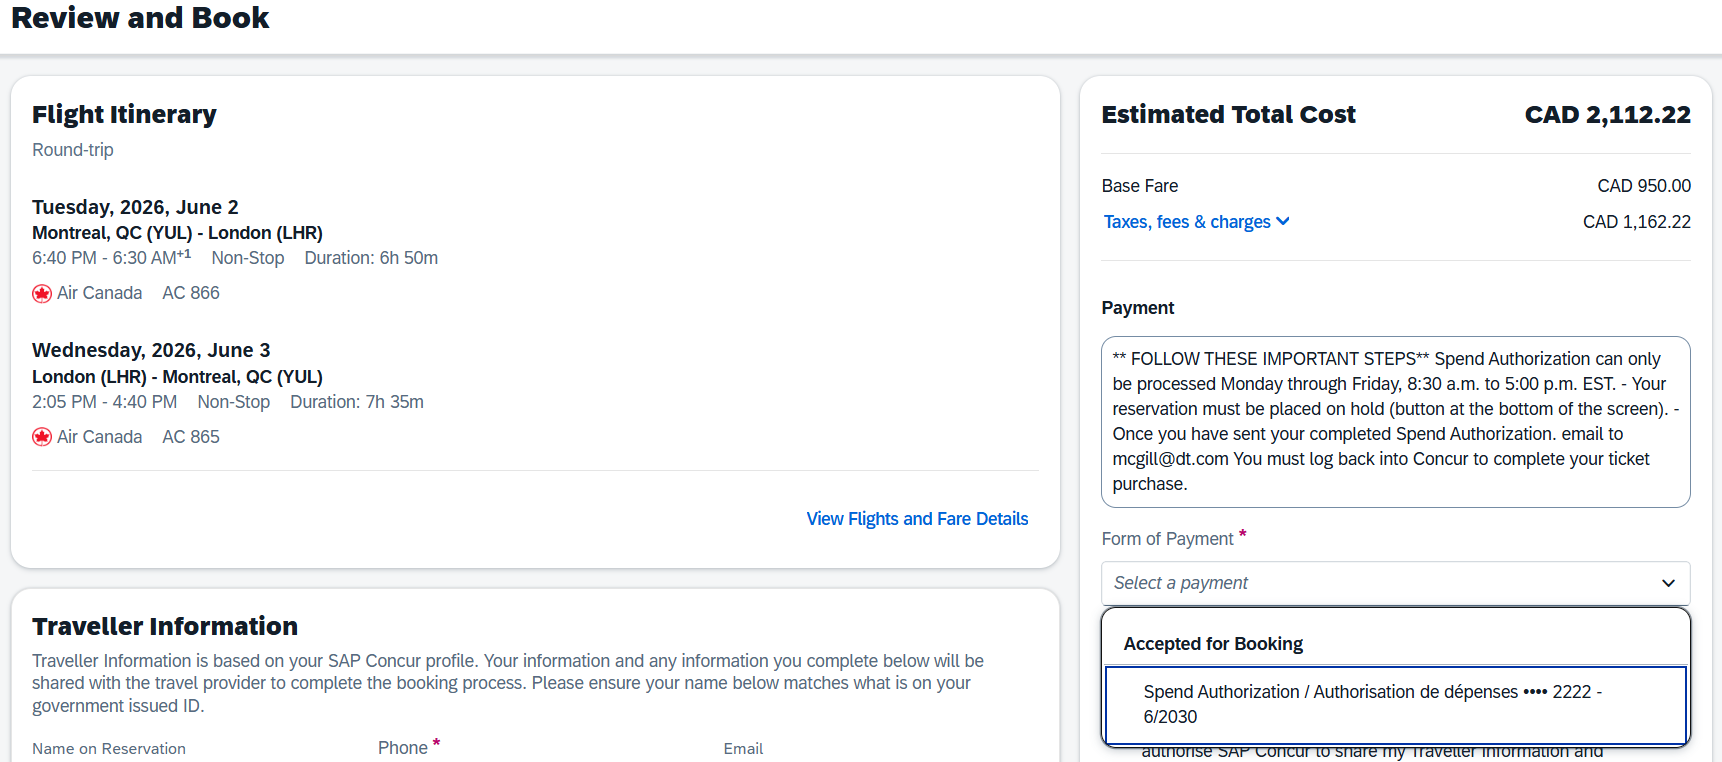
\includegraphics[width=0.7\columnwidth]{Pictures/DropDownMenu.png}
        \end{figure}

        \item Now press ‘Book and Continue’. Note that this does NOT finalize the trip yet. On the next screen, press ‘Hold Trip’. \\
        
        \item You now have 24 hours to have the spend authorization approved by the Finance Service Desk and your supervisor/whoever is paying. To do this, either submit on Workday under the spend authorization section (September – April), or via the Finance Service Desk Jira tool via the link above (May – August). When doing so, you will need to provide evidence of your booking and the cost breakdown. For this, use the flight hold confirmation email you should have received, as well as the screenshot proving your flight was the cheapest option, taken earlier. You will also need your supervisor’s 6 digit research fund code so the spend authorization is charged to the correct account. When approved, you will receive a 7 digit ‘Spend Authorization Number’ that you can input on the final screen. Input this, and then click ‘Finalize Trip’. Your flights are now confirmed. \\

        \begin{figure}[H]
            \centering
            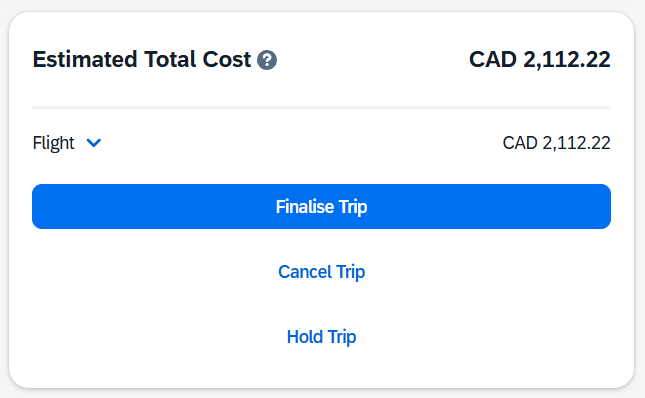
\includegraphics[width=0.5\columnwidth]{Pictures/Finalise.png}
        \end{figure}
        
    \end{itemize}

    \subsection*{Booking flights yourself}
    You would often prefer booking flights yourself, especially if you wish to travel outside of work and spend time visiting places before and after the conference/workshop. The process may seem tiring but it's often the simplest way to book tickets. 
    
    When booking flights on your own, you must provide a \textbf{travel quote} for the event $\pm$ 1 days. Withing \textbf{24 hours} of booking a flight, you need to go to your favourite flight search website such as \href{https://www.skyscanner.ca/}{Skyscanner} or \href{https://www.expedia.ca/Flights}{Expedia} and print the page (Ctrl + P) for travel dates corresponding to the \textbf{\textit{actual dates}} of the conference. The date and time you took the screenshot should be clearly visible at the top. You just need to provide around 10-15 options with various combinations to show that you picked the cheapest option. 
    
    Here's an example that should solve all your queries. 

    \begin{plaincorollary}
    Bob wants to attend a conference in Geneva from $10^{\rm th}-15^{\rm th}$ July. He plans to arrive a day early on the $9^{\rm th}$, so he leaves Montr\'eal on the $8^{\rm th}$. He plans to stay and visit some places in France after the conference and catch a flight back to Montr\'eal from Paris on the $20^{\rm th}$. 

    He books a flight Montr\'eal $\rightarrow$ Geneva on the $8^{\rm th}$ (arriving $9^{\rm th}$) and a return flight from Paris $\rightarrow$ Montr\'eal on the $20^{\rm th}$. This includes his ``leisure'' travel. Suppose this multicity flight costed him \$X. He must also provide a roundtrip airfare \textbf{quote} from $8^{\rm th}$ to $16^{\rm th}$ (one day before and after the conference) from Montr\'eal $\rightarrow$ Geneva. Say this costs \$Y. This is his ``work-related'' travel cost. He will be reimbursed the lower of X \& Y.     
    
    Preferably, he should also provide a quote using other combinations of dates such as $8^{\rm th}$ to $17^{\rm th}$ from Montr\'eal to other surrounding airports like Lyon to avoid the fury of the financial desk. In summary, a travel quote illustrates \textbf{hypothetical work-related expense} and is the maximum he will be reimbursed for.    
    \end{plaincorollary}

    \begin{figure*}[hbt]
        \centering
        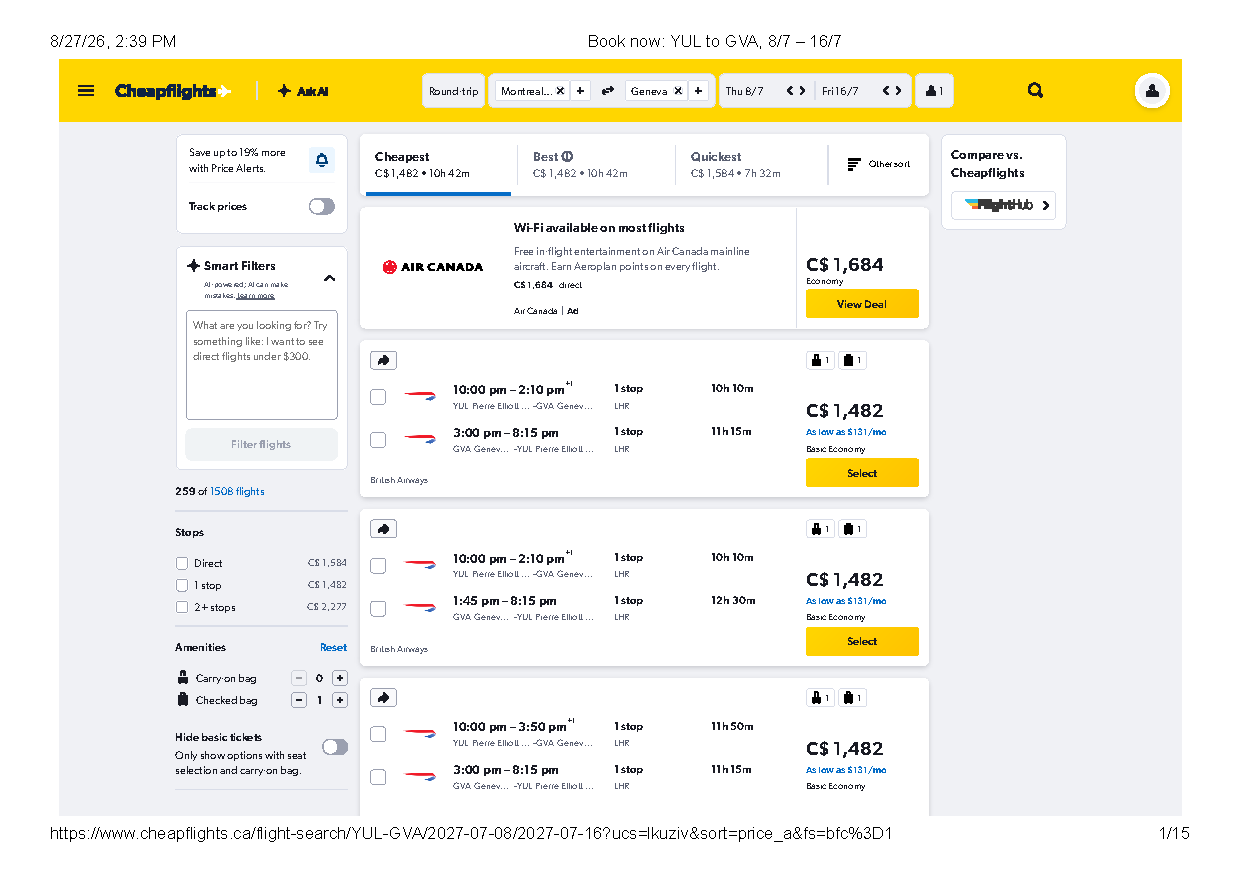
\includegraphics[width=\linewidth]{Pictures/quote.pdf}
        \caption*{A sample travel quote from Montr\'eal to Geneva from $8^{\rm th}$ to $16^{\rm th}$ July. The date and time is clearly visible at the top. The website name is visible at the bottom. The cheapest flight options don't usually include baggage, so checked baggage has been selected on the left.}
        \label{fig:quote}
    \end{figure*}


    \subsection{Food}
    You can either claim a per-diem or provide actual receipts. Usually, per-diems are preferable since the amount is usually higher than what you are expected to spend and also the travel desk doesn't have to scour through your receipts. You must discuss this with your supervisor before embarking on your odyssey. Current per-diem rates are given below (effective May $1^{\rm st}$ 2026). This is the \textbf{maximum} that you are allowed to spend per day on food.

    \vspace{-5 pt}
    \begin{table}[h!]
        \hspace*{-1.7cm}
    \centering
    \renewcommand{\arraystretch}{1.2}
    \arrayrulecolor{ocre}
    \begin{tabular}{|>{\columncolor{ocre!20}}lc|c|}
    \hline
    \rowcolor{ocre!60}
  {\color{white}\sffamily \textbf{Meal}} & {\color{white}\sffamily \textbf{Inside Canada}}  & {\color{white}\sffamily \textbf{Outside Canada}} \\
        Breakfast & \$24 & \$30 \\
        Lunch & \$30 & \$40\\
        Dinner & \$68 & \$81\\
        \hline
        Total & \$122 & \$151\\
        \hline
\end{tabular}
\arrayrulecolor{black}
\end{table}
When filing for reimbursement, you must attach a spreadsheet detailing the days of work travel and the eligible amount for each day. If breakfast is included in your hotel or if dinner is included in the conference reception, you may not be able to per-diem for that item. You can claim a per-diem $\pm 1$ day before and after the conference or workshop.
    
    \subsection{Visas} \index{Travel! Visa}
    MGAPS cannot provide direct visa advice given the diversities in nationalities of the student body as well as variance in the procedures from country to country. Generally, it is recommended that you do your own in depth research and leave plenty of time for any applications and interviews that may be required. If further assistance is required, be sure to contact either the Graduate Program Director (currently Nikolas Provatas, July 2026) or \href{https://www.mcgill.ca/internationalstudents/ihi-contact-us}{International Student Services}.


    \subsection{Travel funding opportunities} \index{Travel! Funding}
    Below is a list of travel awards to consider if you need additional funding for academic travel. Most are field specific, however some are generalized. This list will be continually expanded as we learn of more and more funding opportunities. If you know of any that aren't mentioned here, please get in touch so that we can add it.

   \subsubsection{General}

    \begin{enumerate}
        \item  PGSS Travel Award: \url{https://pgss.mcgill.ca/en/pgss-travel-grants}.
    \begin{itemize}
        \item Provides up to \$750 to cover travel costs.
        \item Award cycles every two months (6 per year).
        \item Can only be awarded once to a given student every TWO fiscal years.
        \item Need to submit letter of intent, letter of reference from faculty and a detailed budget (see website for template).
        \item For the budget, it is recommended that you put much more detail than is required. Justify every expense however small with ample evidence. For example, provide screenshots showing that your flights/accommodation are the cheapest available, or provide links to public transit websites showing fare prices.
        \item Ensure the budget is balanced (total costs and total funding match).\\
    \end{itemize}

    \item  McGill Graduate Mobility Awards (primarily for exchanges): 
    \begin{itemize}
    \item \url{https://www.mcgill.ca/gps/funding/travel}\\
    \end{itemize}

    \item  Physics Department Travel Award:
    \begin{itemize}
    \item \url{https://www.physics.mcgill.ca/grads/travel.html}
    \item \url{https://www.physics.mcgill.ca/grads/gtapp.pdf}
    \item \url{https://www.physics.mcgill.ca/cgi-bin/gta.pl}\\
    \end{itemize}
    
    \end{enumerate}
        
   
    \subsubsection{Nuclear/Particle/HEP}
    \begin{itemize}
        \item \url{https://cinp.ca/junior-scientist-travel-support-program-jsci}
        \item \url{https://cinp.ca/wnppc-graduate-student-travel-awards}
        \item \url{https://cinp.ca/cupc-student-travel-awards}
        \item \url{https://cinp.ca/conference-support}
        \item  \url{https://mcdonaldinstitute.ca/funding-opportunities-2/}
        \item \url{https://mcdonaldinstitute.ca/funding-opportunities/graduate-student-exchange/}
    \end{itemize} 

    \subsubsection{Medical Physics}
    \begin{itemize}
        \item \url{https://comp-ocpm.ca/awards/comp-idea-student-travel-grant}
    \end{itemize}

    \subsubsection{Condensed Matter/Materials/Biophysics}
    \begin{itemize}
        \item \url{https://rqmp.ca/en/call-for-applications/}
    \end{itemize}

    \subsubsection{Astrophysics}

    \begin{itemize}
        \item RADEATE grant. Sponsors 8 weeks of travel and fieldwork, if your supervisor is any of: Adrian Liu, Cynthia Chiang, Jon Sievers, Jason Hessels, Vicky Kaspi, Matt Dobbs + possibly some others (speak to Adrian).
        \item AstroQuébec/CRAQ. Wide breadth of funding opportunities, check \url{https://www.craq-astro.ca/le-craq/nos-programmes-de-bourses/} for updates.
    \end{itemize}

    \subsubsection{Other}
    \begin{enumerate}
        \item  Statistical Society of Canada: 
    \begin{itemize}
    \item \url{https://ssc.ca/en/sources-financement-pour-assister-a-congres}\\
    \end{itemize}
    \end{enumerate}
  \vspace{-10pt}  
    
\subsection{General Links}
\begin{itemize}
   \item Checklist: \url{https://www.mcgill.ca/biology/files/biology/pod1\_expense\_report\_checklist.pdf} (outdated but include a lot of still pertinent information).
   \item Contacts: \href{mailto:sciencefinancepod1@mcgill.ca}{sciencefinancepod1@mcgill.ca}
   \item  Per diem spreadsheet 
        \begin{figure}[H]
        \centering
        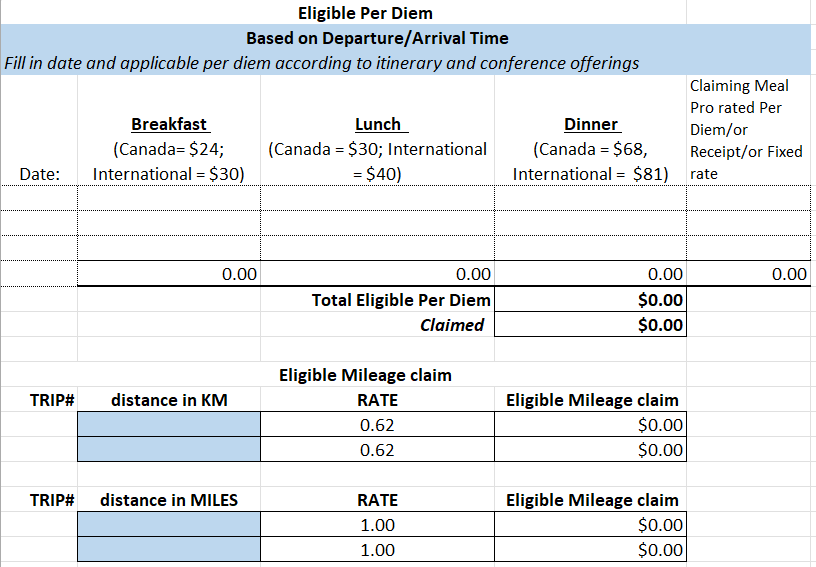
\includegraphics[width=0.7\columnwidth]{Pictures/per diem.png}
    \end{figure}
\end{itemize}

    \section{Reimbursements/Advances} \label{section:reimbursement}\index{Reimbursement} \index{Advance}
    

    \noindent The following section will outline the process of obtaining reimbursement for work-related expenses or conference travel. Most likely, you will need to spend your own money first and then have it reimbursed. It is also possible to get cash advances under certain circumstances, to help offset the financial burden of paying upfront. However, they are only available up to \textbf{30 days} prior to the start of the trip, limiting their usefulness.

    \begin{plaincorollary}
    \noindent Both reimbursements and advances follow a similar procedure. Confusingly, this process changes depending on the time of year. During the regular school year (September to April inclusive), you will have access to the \textbf{\color{ocre} McGill Workday} website to submit the reimbursement/advance. But over the summer, access is annoyingly unavailable, so you must submit a \textbf{\color{ocre}Jira ticket} to the finance desk.
    \end{plaincorollary}
    
\subsection{Workday Reimbursement (Fall \& Winter)} \index{Reimbursement} \index{Workday}

A detailed guide on Workday reimbursement is available on this \href{https://general-knowledgebase.mcgill.ca/spaces/FSKB/pages/124292739/How+to+Create+an+Expense+Report}{\underline{\textbf{link}}}, which has been transcribed here for archival reasons.

\begin{enumerate}[leftmargin=10pt]
    \item Log in to \href{https://wd3.myworkday.com/mcgill/d/home.htmld}{Workday.}\\

    \item On the welcome page, select “Expense Hub”.
        \begin{figure}[H]
            \centering
            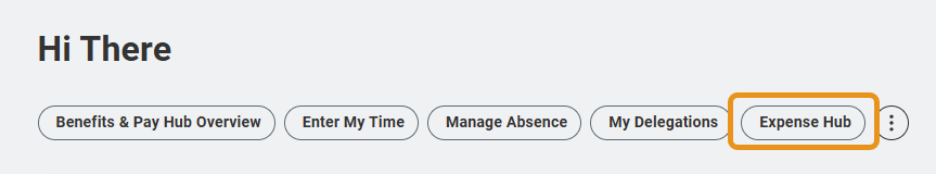
\includegraphics[width=0.8\columnwidth]{Pictures/ExpenseHub.png}
    \end{figure}

    \item Email ingestion information will display. Email ingestion allows employees to upload their receipts directly to their Workday Expenses profile, via a specific email address. Optical Character Recognition (OCR) can accurately read and interpret receipt data to automatically create quick expenses that can be easily added to expense reports. 

    \begin{figure}[H]
            \centering
            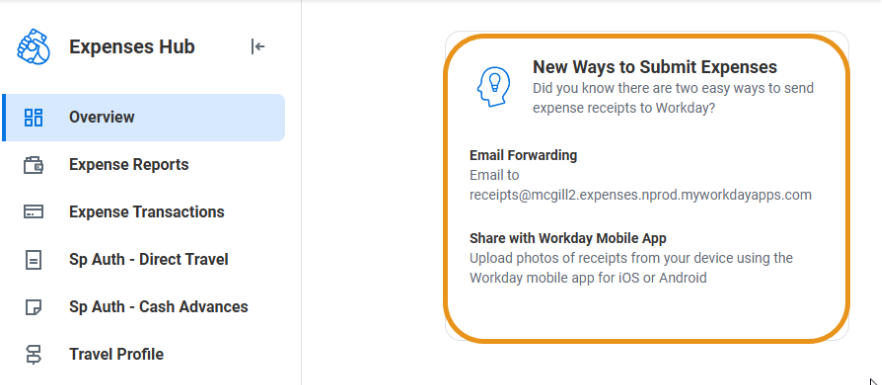
\includegraphics[width=0.8\columnwidth]{Pictures/EmailIngestion.png}
    \end{figure}

    \item Under ‘Tasks’, select “Create Expense Report”.

    \begin{figure}[H]
            \centering
            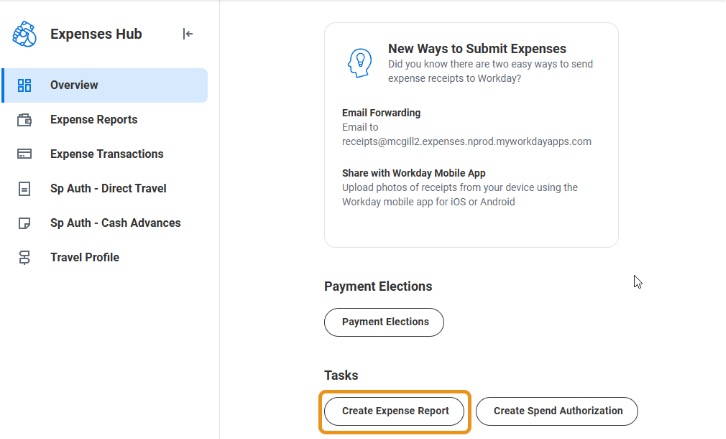
\includegraphics[width=0.8\columnwidth]{Pictures/CreateExpenseReport.png}
    \end{figure}

    \item In the newly opened page, select one of the following options: 
    
    \begin{figure}[H]
            \centering
            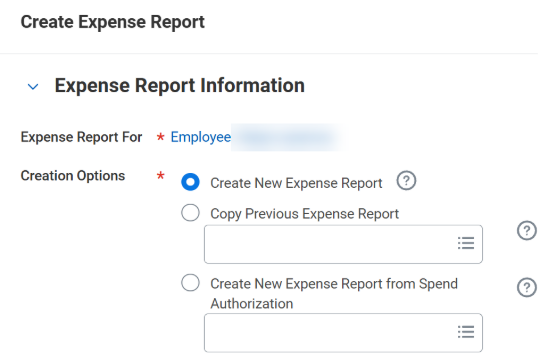
\includegraphics[width=0.5\columnwidth]{Pictures/ExpenseReportInformation.png}
    \end{figure}

    Select the correct option corresponding to your situation as described in the following table:

    \begin{figure}[H]
            \centering
            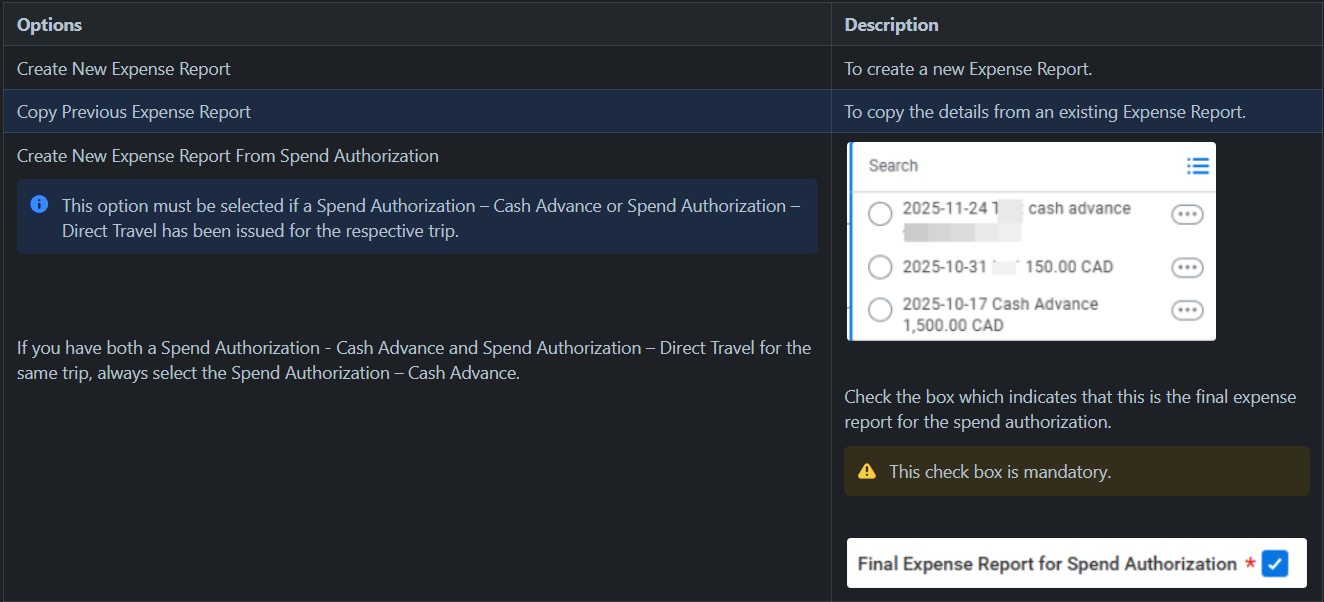
\includegraphics[width=0.8\columnwidth]{Pictures/NewExpenseReportTable.png}
    \end{figure}
    
    \item Continue completing the fields as listed below:

    \begin{figure}[H]
            \centering
            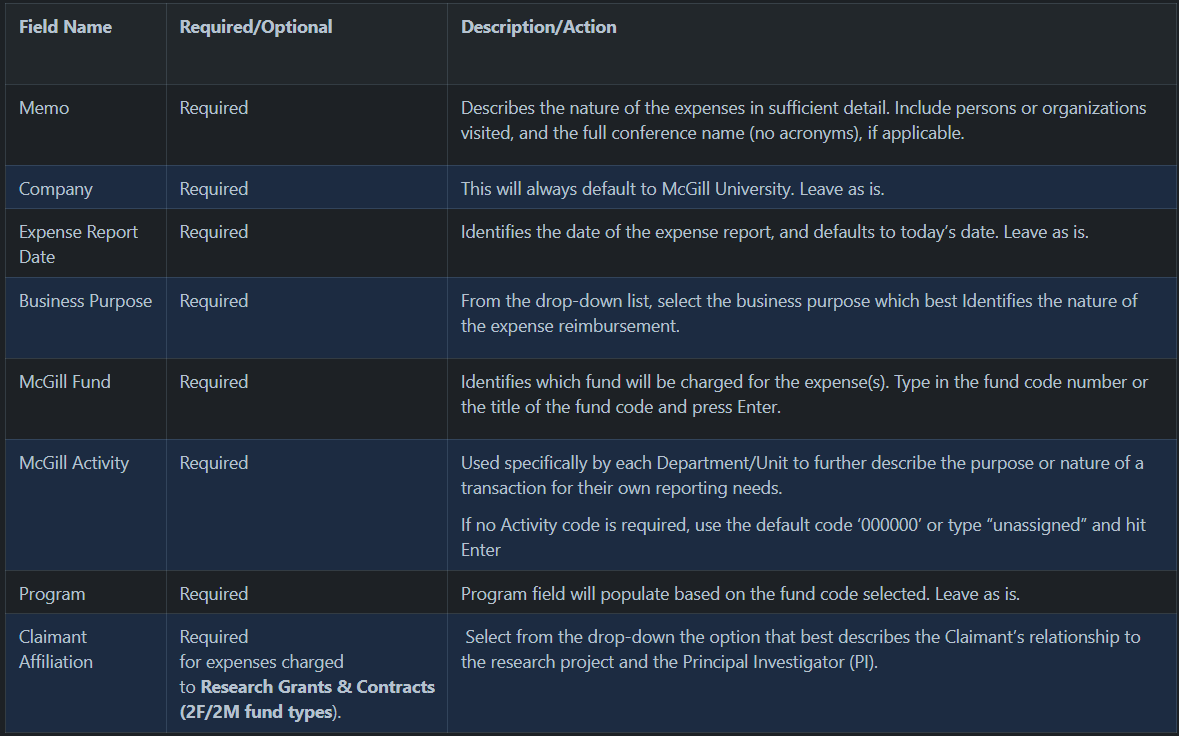
\includegraphics[width=0.8\columnwidth]{Pictures/FormFields.png}
    \end{figure}

    \item If this is the first time you complete an Expense Report for yourself, ensure the Enable Tax field is checked. This is used to calculate and report taxes accordingly. The system will not let you proceed without having this box checked.  All subsequent Expense Reports will automatically have this box checked.\\

    \item If you have uploaded receipts to your profile through email ingestion or the Workday mobile app, they will appear under Quick Expenses. Any expenses charged to a company credit card (i.e. Direct Travel) will appear as credit card transactions. Check off which quick expenses and/or credit card transactions are to be included in the expense report, if applicable.
    
    \begin{figure}[H]
            \centering
        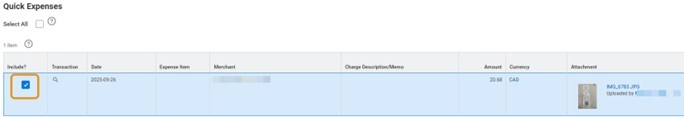
\includegraphics[width=0.9\columnwidth]{Pictures/QuickExpenses.jpg}
    \end{figure}

    \item If no quick expenses or credit card transactions are to be included in the expense report, proceed to step 10.\\

    \item Once this first page is complete, click \textbf{OK}. The information entered will serve as the Header of the Expense Report.\\

    \item   A unique expense report number will be generated, EXP-00000XX. The name of the employee will also display, as well as the status of the Expense Report, if any cash advance is applied, amounts previously paid by the university (i.e: to Direct Travel) and the reimbursable amount. These last fields will automatically update as expense items are added.\\

    \item The next step is to click ‘Add’ to add new expense lines. You can also add additional quick expenses or credit card transactions if available/uploaded in your profile.\\

   \item If you are adding a new expense, proceed to step 14. If quick expenses were included from the header page, separate expense line items will be created for each and will populate some of the information from the receipt, along with the receipt(s) as attachment(s). Complete the remaining fields as listed in step 16.\\

   \item The following page will display:

    \begin{figure}[H]
            \centering
            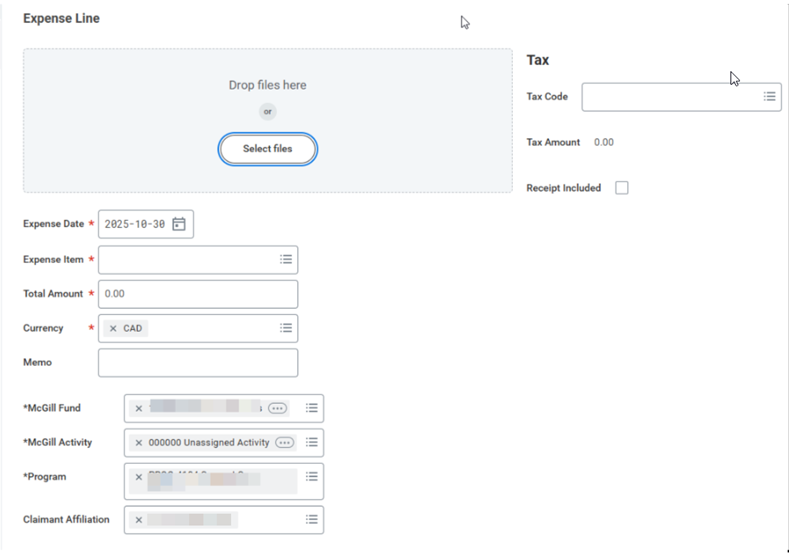
\includegraphics[width=0.65\columnwidth]{Pictures/ExpenseLine.png}
    \end{figure}

    \item Attach the receipt or a copy of the receipt by either dropping the respective file in the attachment section, or by clicking “Select Files” and selecting the appropriate receipt. This is mandatory, and the expense report cannot be submitted without each expense line item having a corresponding attachment. Receipts are not required for the following expense items: meal per diem, lodging allowance, childcare per diem, mileage, tolls, public transportation and gratuities if paid in cash. \\

    \item In the Expense Line section, update/complete the expense item fields as per the information indicated below:

    \begin{figure}[H]
            \centering
            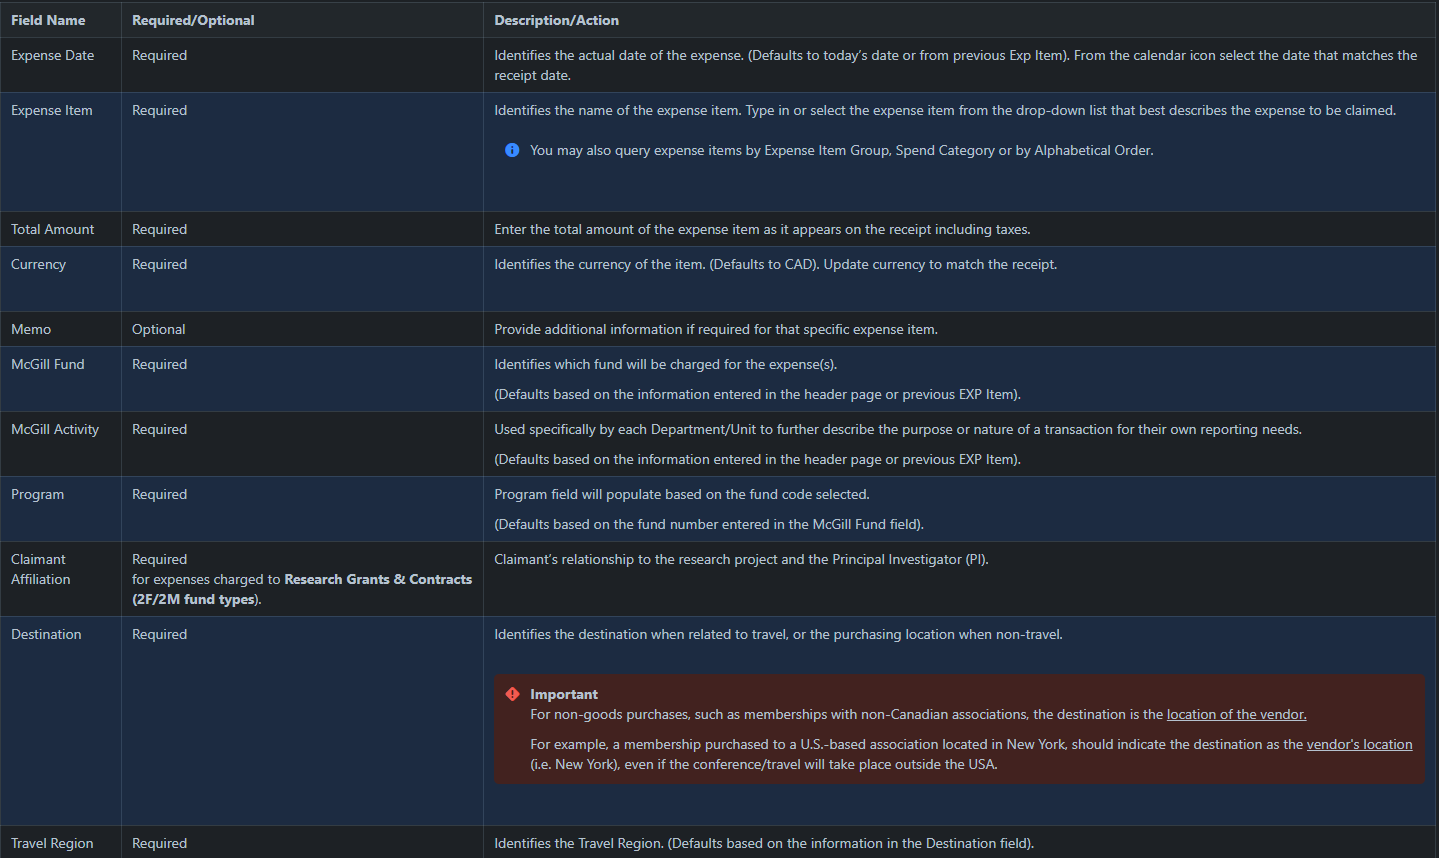
\includegraphics[width=0.8\columnwidth]{Pictures/FormFields2.png}
    \end{figure} 

    \item The tax code and tax amount will populate based on the information entered in the Item Details section. As advised and recommended by McGill University's tax consultants, McGill University has implemented the "factor method" in Workday Expenses. The "factor method" is a tax calculation approach that uses a predetermined factor, therefore tax calculation displayed in WD Expenses may differ from the taxes displayed on receipts. All tax calculations in Workday Expenses (except for airfare, train, chartered bus and seat selection) must NOT be overridden. \\

    \textbf{\color{ocre}Important:} The taxes are only to be overridden to match what is indicated on the receipt for the following expense items: airfare, bus chartered, seat selection fees and train. \\

    \item Should additional expense lines be required, click on “Add”. Repeat steps 12-17 as needed. If alerts and/or error notifications display, click on the notification to expand and read the message. Click on the ‘X’ to exit the alert/error message. 

    \begin{plaincorollary}
 \textbf{\color{ocre}Tip:} The following receipts may be grouped by purchasing location and entered as a single item:
    \begin{itemize}
        \item Parking
        \item Gas
        \item Taxi - if travel related. Local (Montr\'eal) taxi receipts for McGill staff must be entered as individual items with a detailed explanation for each receipt.
        \item Per Diem
        \item Postage
        \item Tolls
        \item Calling cards
    \end{itemize}   
    \end{plaincorollary}
    

    \item Once all expense lines have been entered, select one of the following options below:

    \begin{figure}[H]
            \centering
            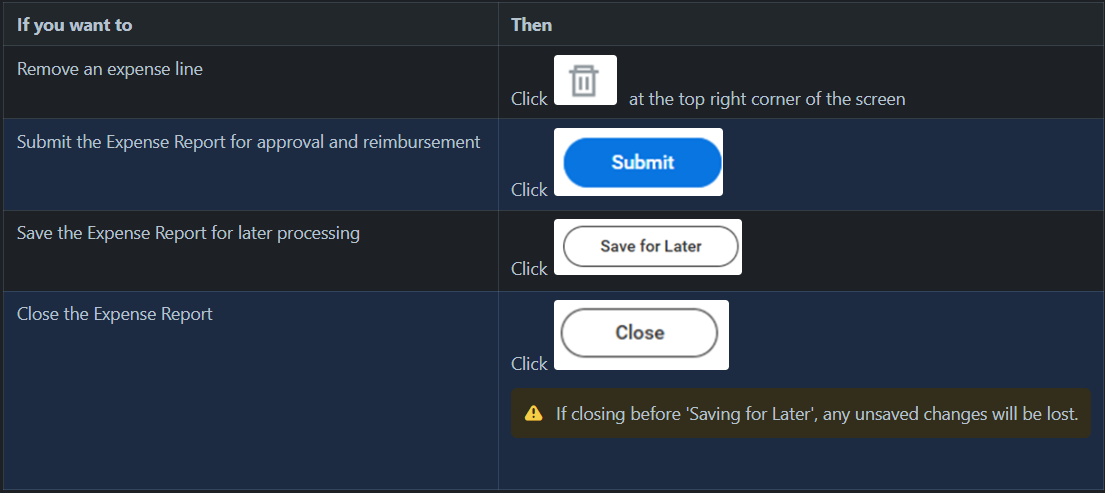
\includegraphics[width=0.8\columnwidth]{Pictures/Step19.png}
    \end{figure}
    \item  Once the expense report is submitted, a message will display to indicate the expense report was successfully submitted, and routed to an Expense Partner’s approval’s queue.

    \begin{figure}[H]
            \centering
            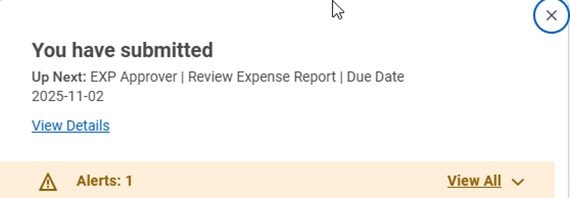
\includegraphics[width=0.8\columnwidth]{Pictures/ReportSubmitted.png}
    \end{figure}

    \item Once the expense report is reviewed and approved by all approvers (Expense Partner(s) and FFM(s)), the expense report is settled for payment.\\
    
\end{enumerate}    

    
    \subsection{Jira Ticket (Summer)} \index{Reimbursement} \index{Jira Ticket}
    \noindent A great step by step tutorial for the Jira ticket process is available at the   \href{https://general-knowledgebase.mcgill.ca/spaces/FSKB/pages/133300374/Student+Grad+Undergrad+-+How+to+Submit+an+Expense+Report}{McGill General Knowledge Base.} The guide is for an expense reimbursement, but the procedure for a cash advance is nearly identical. A guide for the Workday process follows this one. The guide has also been transcribed here for archival reasons.
    
    \noindent As a student, you must complete and submit the Student Expense Reimbursement JIRA form via the Finance Service Desk Portal: \url{https://hrservicedesk.mcgill.ca/servicedesk/customer/portal/12}.
    
    \noindent Before you begin the reimbursement process, make sure you have the \textbf{fund number, activity code, supporting documents} and \textbf{receipts} and the \textbf{name of your supervisor/Principal Investigator}. Also ensure that your banking information is up to date on Minerva. Refer below to additional information on these required data.

     \noindent \textbf{Fund Number:} Six-digit code that should be provided by your supervisor/Principal Investigator prior to incurring “other” expenses, including travel.
     
     \noindent \textbf{Activity Code:} Also provided by your supervisor/Principal Investigator. If none is provided, use the default code: 000000.

    \noindent \textbf{Supporting documents/receipts:} Required for all expenses being claimed except for mileage claims, meal per diems, tolls, public transportation and gratuities if paid in cash. All receipts must include:
    \begin{itemize}
        \item Identification of the supplier
        \item Supplier’s GST and QST number, when applicable
        \item Name of claimant, when applicable (e.g., hotel, airfare, registration)
        \item Full description of expense
        \item Total amount paid, along with proof of payment indication.\\
    \end{itemize}
     
     \noindent \textbf{\color{ocre}Note:} If you have received a travel award, submit only the portion of your expenses that exceeds the amount of the award (for example, if your travel award was \$500 and your total expenses were \$1,000 you should only submit the remaining \$500). If your total expenses are less than the amount of the award, do not submit an expense report. Instead, contact your Graduate Program Coordinator (GPC) to arrange for the unused funds to be returned to the university.\\
     
    
    \begin{plainexercise}
    \textbf{\sffamily \normalsize As per the Travel and Other Expenses Policy:} 
           
    Expense reports related to travel, trips (including field trips) and conferences must be submitted no later than \textbf{30 days} following the return date. 
    
    Expense reports not related to travel, trips (including field trips) or conferences that are submitted after \textbf{90 days} following the oldest receipt date will not be reimbursed.
    \end{plainexercise}


 

    
     \noindent \textbf{\sffamily Step-by-step Instructions}

     \begin{enumerate}[leftmargin=10pt]
         \item Log in the \href{https://hrservicedesk.mcgill.ca/servicedesk/customer/portal/12}{Finance Service Desk Portal.}\\

         \item Under `McGill Student (Grad \& Undergrad) Expense Reimbursements \& Spend Authorizations', select the Expense Reimbursements request form. If you're applying for a cash advnce instead, select the Cash Advance form instead.

            \begin{figure}[H]
                    \centering
                    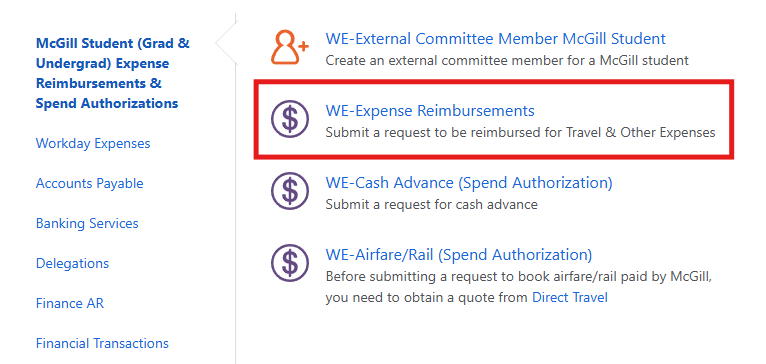
\includegraphics[width=0.8\columnwidth]{Pictures/Expense_Reimbursement.png}
            \end{figure}
            
        \item Select that you are completing this request for yourself.\\

        \item Select your student status, i.e., Graduate or Undergraduate.\\

        \item Select if you received a travel award. Note: If yes, upload the travel award confirmation letter in the Attachment section.\\

        \item Provide a brief description of your reimbursement request, e.g., “NAME OF CONFERENCE -November 2025”.\\

        \item Type in and select the name of your supervisor/Principal Investigator.\\

        \item Enter the 6-digit fund code provided by your supervisor/Principal Investigator. If you need to charge more than one fund, use the Expense Description box to indicate the distribution of expense amounts to each fund, enter the additional fund codes, along with their respective activity codes.\\

        \item Enter the activity code to be charged for all expenses. If it’s unknown, use 000000.\\
    
        \item Select the reason for your request by selecting from the drop-down menu in the Purpose of Expense field.\\
    
        \item Choose the start and end date of your expense/travel by clicking the calendar icon.\\
    
        \item Indicate if this trip/travel included personal dates/travel. Note: If you select yes, provide the dates/expenses which are not related to university-related travel in the respective field.\\
    
        \item Enter your destination (city, province/state). For non-travel related expenses, please enter Montr\'eal, Qu\'ebec.\\
    
       \item Select the destination country from the drop-down menu.\\

       \item In the Expense Description field, provide details of the expense, such as:
    \begin{itemize}
        \item Complete name of the conference, purpose, etc.
        \item Indicate any amounts not to be reimbursed, e.g., personal amounts, travel awards coverage.
        \item If you need to charge more than one fund, indicate the distribution of expense amounts to each fund, enter the additional fund codes, along with their respective activity codes.For more information, refer to section PR7.1.8 of the \href{https://www.mcgill.ca/financialservices/policies/reimburse/procedures}{Procedures for Travel \& Other Expenses.}\\
    \end{itemize}

        \item Attach all receipts or clear photos of receipts pertaining to the expenses for which you are claiming reimbursement.Note: Upload each receipt separately. Do not combine all receipts in 1 PDF.
    
    \begin{itemize}
        \item In the case of airfare with costs that are not necessarily a consequence of travel on behalf of McGill, a quote for the itinerary purely related to the university business must also be attached.\\
    \end{itemize}

        \item Acknowledge that your banking information is up to date on Minerva; all expenses claimed are accurate complete and legitimate; and, that any false or misleading claims may result in an obligation to return the funds to McGill University.\\

        \item Click the Create button. A ticket with its respective number will then be generated. You will also receive that information by email.\\
        
     \end{enumerate}

  
    
    \noindent \textbf{\sffamily What to expect after submitting a claim?}
    
    The claims will be processed by Finance Service Desk and approved by your Faculty/Administrative Unit’s Expense Partner, who will be added to the ticket. This will happen in Workday Expenses, and you will be notified when it happens. If the Expense Partner requires additional information from you, they will use the ticket to communicate with you. Ensure you monitor your inbox and/or the ticket in the link provided to avoid any delays in processing the claim. Once the Expense Partner reviews and approves the claim, the expense report is en route to the supervisor(s)/Principal Investigator(s) responsible for the fund(s) being charged for approval. Once all approvals are recorded, you will receive an email notification that the funds will be deposited into your bank account within 48 hours, and the ticket will be closed in the Finance Service Desk Portal.
    
    

\section{Stipend and Tuition} \index{Stipend} \index{Tuition}
The most up to date information about tuition and financing can be found on the McGill Physics \href{https://www.physics.mcgill.ca/grads/finance.html}{website}.

As of the 2026/2027 academic year, the net annual tuition fee for a McGill Physics graduate student is {\color{ocre}\$5,722.05} (\$3,321.83 + \$2,400.22) and {\color{ocre} \$6,435.31} (\$4,035.09 + \$2,400.22) for International Students after departmental subsidies for non-Québec students.

There are certain fees that are opt-outable when you go on \textit{Minerva > Student Menu > Student Accounts Menu > Student Fee Opt-outs}. Opt out period is limited to the two weeks prior to the fee payment deadline in September and in late January. Check \href{https://www.mcgill.ca/student-accounts/tuition-fees/fee-descriptions}{the fee descriptions} to understand your fees and make an informed decision on whether to pay them or not.

Typically, a Physics student receives financial support in the form of a stipend and teaching assistantship income (see section \hyperref[TA]{\textcolor{purble}{\ref*{TA}}}).

For the 2026/27 academic year, non-scholarship students will receive a stipend of {\color{ocre}\$27,061}, contingent upon satisfactory progress toward the degree, within the normal time frame for its completion. Students holding an external award or scholarship that is less than \$27,061 will receive a stipend such that the total of the scholarship and the stipend is \$27,061.

\subsection*{TA-ship income} \index{Teaching Assistantship}

Graduate students may apply for TAships of approximately \$6,922 totalling 180 TA hours over the course of the academic year. The conditions of TAships are governed by a collective agreement, and graduate students are considered to be in a ‘priority pool’ for the first two years of their MSc program, and the first five years of their PhD program. TAships are not compulsory, and while the department typically is able to offer TAships to all priority pool students, this cannot be guaranteed.
    

\section{Scholarships and Awards} \index{Scholarships}\label{section:scholarships}
Some common sources of funding are listed below.

\subsection{Natural Sciences and Engineering Research Council of Canada (NSERC)} \index{Scholarships! NSERC}
\begin{itemize}
    \item \href{https://nserc-crsng.canada.ca/en/funding/funding-opportunity}{All funding opportunities}
    \item \href{https://nserc-crsng.canada.ca/en/funding-opportunity/canada-graduate-research-scholarship-masters-program}{Canada Graduate Research Scholarship - Master's program} -- December 1st deadline
    \item \href{https://nserc-crsng.canada.ca/en/funding-opportunity/canada-graduate-research-scholarship-doctoral-program}{Canada Graduate Research Scholarship - Doctoral program} -- Check McGill's \href{https://www.mcgill.ca/gps/funding/fac-staff/awards/tri-agency-cgrs-d-cihr-nserc-sshrc}{internal deadline} (typically mid September)
\end{itemize}

\begin{plainexercise}
    If you apply for NSERC CGRS D as a McGill student, you must go through the internal application process first because McGill has a doctoral award quota. The internal deadline is typically a month earlier than the Direct To Agency deadline. You will be notified if your application is selected to be forwarded to the federal level.
\end{plainexercise}

International students enrolled in Canadian institutions are eligible to apply for NSERC CGRS D but only up to 15\% of the available awards can be allotted to them.

If you enter into the doctoral program straight from Bachelor's, consider applying for the NSERC CGRS M for your first year to maximize your funding period.

Consult the eligibility criteria for your desired scholarship carefully. In general, the eligibility windows are:
\begin{itemize}
    \item Master's students -- for CGRS M: 0 to 12 months of full time studies in the MSc program
    \item Direct entry PhD students (from a Bachelor's program):
        \begin{itemize}
            \item For CGRS M: 0 to 12 months of full time studies in the PhD program
            \item For CGRS D: 0 to 36 months of full time studies in the PhD program
            \end{itemize}
    \item PhD students after obtaining a MSc -- for CGRS D: 0 to 36 months of full time studies in the PhD program
    \item PhD students fast-tracked from a MSc program: 0 to 36 months of full times studies in the PhD program (meaning, the counter only starts when you officially become a PhD student).
\end{itemize}

The well-known secret of this system is that you can start applying for NSERC scholarships the year prior to the start of your program. For example, a student entering the MSc program in Fall 2027 can apply for NSERC CGRS M in Fall 2026. However, you can only apply for NSERC CGRS D at most three times. 
    
\subsection{Fonds de recherche du Québec (FRQ)}\index{Scholarships! FRQ}
    \begin{itemize}
        \item \href{https://www.mcgill.ca/gps/funding/intl/provincial-agency-awards}{Master's Research Scholarships}
        \item \href{https://www.mcgill.ca/gps/funding/intl/provincial-agency-awards}{Doctoral Research Scholarships}  
    \end{itemize}
\begin{plainexercise}
    Unlike NSERC, FRQNT applications are submitted directly to the agency at \href{https://frqnet.frq.gouv.qc.ca/}{FRQnet}. However, McGill requires that students complete a FRQ application details \href{https://www.mcgill.ca/gps/funding/intl/provincial-agency-awards}{form}. 
    
    The abstract for your application must be submitted in French. McGill's GPS offer the translation service on a rolling deadline basis, consult \href{https://www.mcgill.ca/gps/funding/intl/provincial-agency-awards/preparing-frq-doctoral-competition}{this page}.
\end{plainexercise}
The eligibility window for FRQNT is quite similar to NSERC (more details are provided above), with a small nuance of FRQ counting full-time study terms instead of months (3 terms instead of 12 months, and 14 terms instead of 36 months). The deadline is usually \textbf{October 1st}.

\subsection{Internal Scholarships} \index{Scholarships! Internal}

You will receive an email with detailed instructions around May each year.

\subsection{Other scholarships} \index{Scholarships! Others}
\begin{itemize}
    \item \href{https://www.mcgill.ca/gps/funding/opportunities/masters}{Master's students} 
    \item \href{https://www.mcgill.ca/gps/funding/opportunities/phd}{PhD students} 
    \item \href{https://www.mcgill.ca/studentaid/scholarships-aid/graduate}{All graduate students}
\end{itemize}

\begin{plainexercise}
    McGill holds fellowship information sessions for major awards, usually around August every year. It is a good opportunity to come ask questions and get tips on crafting a good application. Check this \href{https://www.mcgill.ca/gps/funding/maximize-my-chances/workshops-information-sessions-and-webinars}{page}.
    
    Also keep an eye out in your McGill email inbox for information about application workshops and reviews.
\end{plainexercise}

Beyond the scholarships listed above, it is also possible in some cases to apply to privately funded scholarships, such as the \href{https://www.janestreet.com/join-jane-street/programs-and-events/graduate-research-fellowship/}{Jane Street Graduate Research Fellowship}. These scholarships will frequently be advertised in your emails, though it may be the case that some you might have to personally search for depending on your specific research and situation.

\subsection{Top-ups} \index{Top-ups}
All students holding a scholarship/award of a value less than \$40,000 per year receive an award top-up bonus, in addition to the stipend described above. Holders of NSERC and FRQNT scholarships with a value of less than \$30,000 per year receive an award top-up bonus of \$6,500. Holders of other scholarships and awards will receive an award top-up bonus equivalent to 20\% of the value of their awards, up to a maximum total amount of award plus top-up of \$40,000. Top-up bonus for holders of scholarships and fellowships of a value greater than \$40,000 is left at the discretion of the supervisor.

If the scholarship or fellowship includes an amount to cover the extra tuition fees paid by international students, that amount will first be subtracted before calculating the top-up.

    
    \section{Personal finances} \index{Personal Finances}
Personal finance is extremely important to set yourself up for success in the future. The reality is that most grad students don't make much money so having clear financial planning can also be a matter of survival.

We recommend going through \href{https://mcgillpersonalfinance.com/}{this free online} course offered by McGill for the foundation of budgeting, saving, and investing. In this section, we take a deep dive into the world of finance to give you at least the confidence to take the next steps of optimizing your finances. We try to address all the commonly asked questions about finances from years of mentoring new students settling in Canada/Montr\'eal.

\textbf{\color{ocre}Disclaimer:} The author is just a physics graduate student who happens to be very interested in personal finance and, therefore, volunteered to write this guide. They don't have formal financial advising accreditation so take their words as mere suggestions and do your due diligence in verifying the following information. 

\subsection{Banking} \index{Banking}
Banking in Canada is very well regulated. Therefore, there is really no wrong choice in picking a bank in Canada (as long as it's a reputable institution, your money will be safe). 

There are 3 categories of options:

\subsubsection{Traditional brick and mortar banks
}

The Canadian banking sector is dominated by the Big Five banks: Royal Bank of Canada (RBC), Toronto-Dominion Bank (TD), Bank of Nova Scotia (Scotiabank), Bank of Montr\'eal (BMO), and Canadian Imperial Bank of Commerce (CIBC).

There is very little to differentiate between them in terms of experience, fees, and perks. They all have branches close to McGill. You can choose based on vibes and it won't make much of a difference. Often, they will run a promotion for opening an account with them (i.e. get a free ipad/ipod/mac) so choose one with the best offer at the moment.

The nice thing about them is that you have physical branches all over country to walk into and talk with a real person. However, they are slow to innovate and tend to have higher fees and fewer rewards as compared to their online competitors.

\subsubsection{Credit unions
}

A credit union is a member-owned nonprofit cooperative financial institution, and they tend to offer very similar services to a bank. They have more of a local feel to them, and the services tend to be more personable. The biggest one in Québec is Desjardins. 

\subsubsection{Online-only banks}

This is where it gets interesting. They offer no fee banking and higher saving interest rates than a traditional bank. The limitation is that you don't have a physical branch (but how often do you need to go to a bank anyway?) and online support (phone, email, chat) can be frustrating.

Some options that work in Québec:
\begin{itemize}
    \item \href{https://www.wealthsimple.com/en-ca}{Wealthsimple}: It is a fintech platform that is quite popular, especially to young Canadians, for its simple no-fee investing tools and high baseline interest chequing accounts. Their accounts are free to open, they reimburse ATM fees for cash withdrawal, their cash card has no foreign exchange (FX) fees. They also offer a good credit card but (or plus, depending how you feel) they gamify saving and investing through frequent giveaway contests. They also run a great pay-what-you-can online tax filing service.
    \item \href{https://www.eqbank.ca/ }{EQ Bank}: They consistently offer the best interest rates for your savings/chequing account. They also reimburse ATM fees. Their cash card has no FX fees while giving 0.5\% cashback on transactions.  
    \item \href{https://www.tangerine.ca/en/personal}{Tangerine}: They are a subsidiary of Scotiabank, but they operate independently. They offer full daily banking suites (meaning you get a true debit card, unlike the above two) and attractive (but for a limited time) promo rates for their saving accounts.
    \item \href{https://www.pcfinancial.ca/en/pc-money-account/}{PC Money Account}: This is linked to one of the biggest grocery reward programs in Canada. They have high saving interest rates, no FX fees, no monthly fees, and spending cashback in the forms of reward points. 
\end{itemize}

\begin{plaincorollary}
    These digital banks often run promotions for account opening as well. Reach out to fellow graduate students for referrals for extra perks.
\end{plaincorollary}


\subsection{Credit Cards} \index{Credit Cards}
In Canada, a credit score is used to determine your likelihood of repaying a loan. You need it to get a mortgage, finance a car purchase, or in some cases to rent a place so it is important to start building your credit history in Canada early especially if you are planning to work and live in Canada in the long term. The easiest way to do so is by obtaining a credit card and using it responsibly.  

You can read up on credit score and report in Canada \href{https://www.canada.ca/en/financial-consumer-agency/services/credit-reports-score/credit-report-score-basics.html}{here}. Note that you can view your credit reports for free from Canada's main credit bureaus, Equifax and TransUnion. Furthermore, as a Québec resident, you have the right to lock and unlock your credit reports to prevent identity theft.

All that said, if you don't have good financial habits (ie. you tend to spend more than you have), credit cards can be dangerous to your financial future. 

Alright, let's dive right into the world of credit cards!

\subsubsection{Must know about credit card use}
If you've never gotten a credit card before, it is very important to understand how it works to maximize rewards and avoid fees. Here, we will outline the few must know basics, but you can get more details \href{https://www.canada.ca/en/financial-consumer-agency/services/credit-cards/credit-card-work.html}{here}. 

Your billing period is typically a month (28 -- 31 days). All the transactions you made in that month will count toward your owing balance on your statement at the end of the period. You will then have at least 21 days of interest free grace period (per federal regulations) to make your payment. \textsc{\color{ocre}You must make your payment in full to avoid any interest charges.} Credit cards typically charge very high interest rates (19\% to 29\% annually, compounding daily!) so a missed or partial payment means that you must pay exorbitant interests on every purchase you made for that whole period until it is paid off.

Scary! How do you avoid this? We recommend \textsc{\color{ocre} setting up automatic payment for your credit card}! If you wish to pay manually, you still can -- the autopay only kicks in at the end of the grace period if you have not paid your balance in full, so it helps you avoid any interest fees. In fact, it makes mathematical sense not paying manually and letting autopay do its job because the money you leave in your chequing account can keep accumulating saving interests (the good kind!) during the grace period. However, it is a good idea to look at your statement once a month to check for any unauthorized transactions and understand how much you've spent!

The caveat is of course to make sure you have enough money in the account to which you link the autopay to avoid any non-sufficient funds (NSF) fee.

You'll have a certain credit limit, ie. the maximum amount you can borrow at any given time. If you have no credit history, your limit will be very low. So, you might need to pay it off more often to continue using it throughout the month. Or you might have to ask for one-time limit increase to make big purchases (for example, to pay conference registration fees). 

{\color{ocre}Important}: Avoid cash advances or cash-like transactions (essentially getting cash from your credit card!) because the interest rate is astronomically high and there is no grace period for them. Don't spend what you don't have to begin with but if desperate, look into student loans or low interest lines of credit from your bank first. 

\subsubsection{Your first credit card}
If you are new to Canada, you can get a Newcomer or Student credit card from any traditional bank you open an account with. Sometimes, the bank might require an in-person appointment to approve your first card. A secured card (you put money in the card before you can use, so functionally more like a debit card) can also be a good starter, especially if you don't know if you can use a credit card responsibly.

These “beginner” cards don't have super exciting perks so there is not much differentiation between cards. The purpose of your first card is simply to build your credit history here then you can get better cards down the line (if you want).

If you have a banking history but not necessary credit history in Canada (as in you have an account with the same bank since forever but never had a credit card before), you might be able to talk to your bank to get a more decent credit card. In such case, you can try for the cards in the next section first.

If you have/had an American credit card (especially AMEX), it's worth checking with your Canadian bank if they can open for you a good card by pulling your American credit history. 

Some decent student credit cards (as of Aug 2026) to consider:
\begin{itemize}
    \item BMO CashBack Mastercard for Student -- no annual fee, 3\% cashback on groceries, 0.5\% for other purchases
    \item Desjardins Cash Back Mastercard/Visa -- no annual fee, 2\% cashback on dining, entertainment, alternative transportation and pre-authorized payment, 0.5\% otherwise
    \item RBC Cash Back Mastercard -- no annual fee, 2\% cashback on groceries, 1\% otherwise after the first \$7000 spent per year.
    \item Scotiabank Scene+ Visa Card (for students) -- no annual fees, 2 Scene points per \$1 spent for certain grocery stores, home hardware stores, and Cineplex, 1 Scene point per \$1 otherwise (1 Scene point is valued at 1 cent per point)
    \item CIBC Dividend Visa Card for Students -- no annual fees, 2\% cashback on groceries, 1\% on certain categories
\end{itemize}

\subsubsection{Good general credit cards}

If you're in the category of "just make it simple" user, cashback cards are the easiest because you don't have to think about maximizing your point redemption. The author recommends having a Visa and a Mastercard, which will cover the majority of use cases and serve as a backup for each other. AMEX has some very nice cards as well but in Québec, its acceptance rate remains quite low, so check that the places you frequently shop at would accept it before getting one.

In general, knowing how much you spend per month (by tracking your spending a few months after moving to Québec) helps you select the best card for yourself. For example, if your biggest expense is usually groceries, you can choose a card with high cashback on groceries. 

You could of course get multiple cards that reward different categories if you are keen on maximizing your returns. There is a tradeoff between simplicity and profits so it's up to you what you want.

Also, don't be afraid to get a credit card with an annual fee if the maths works out (but don't go crazy paying for multiple high fee cards). 

Another thing to look for when choosing a credit card is insurance such as extended warranty and travel insurance. If you often rent a car for weekend trips, car rental insurance could save you hundreds in not having to purchase insurance add-ons.

One caveat is that cards with fees usually require a minimum income so you might have to first establish a banking relationship with an institution then talk them into giving you the card you want. One possible maneuver is “upgrading” your existing no fee card.

There are simply way too many credit cards to highlight in this little guide section. So we recommend reading these 2 Globe \& Mail articles:
\begin{itemize}
    \item Guide for people interested in \href{https://www.theglobeandmail.com/business/article-cash-back-credit-cards-guide-canada/?utm_medium=RedditAd%20and%20utm_campaign=traffic_mkt}{cash-back cards}.
    \item Guide for people interested in \href{https://www.theglobeandmail.com/business/article-travel-credit-cards-guide-canada/?utm_medium=RedditAd%20and%20utm_campaign=traffic_mkt}{travel cards} (ie. good for travel perks)
\end{itemize}

You can also use \href{https://www.finlywealth.com/credit-cards/compare}{this tool} to filter out credit card that best suits your usage.

That said, here are a few underrated credit cards:
\begin{itemize}
    \item \textbf{Rogers Mastercard:} No annual fee, 1.5\% on everything (if not a Rogers customer) or 2\% on everything and 5\% on Rogers services as a Rogers customer. The World Elite version has comprehensive insurance (but notably no travel insurance).
    \item \textbf{Wealthsimple Visa:} No foreign exchange fee, 2\% on everything, comprehensive insurance (but notably no car rental insurance). Annual fee is waived under certain conditions. 
    \item \textbf{Canadian Tire Triangle Mastercard:} No annual fee, 3\% on groceries, 1\% otherwise as CT money to use in their stores. You can pay a lot of bills through their portal to earn 1\% back on bills you normally can't pay with a credit card (tuition for example!). Similarly, the World Elite version has comprehensive insurance and free roadside assistance (especially good if you plan to drive during Canadian winter!) 

\end{itemize}

    The first two are great options if you just want to use one card for everything. 

\subsubsection{Play the credit card game}

    No, we're not talking about credit card churning (it's a whole different beast!). We're talking about getting money / points back for every cent you spend, especially for bills that take up a big percentage of your monthly expenses that you normally can't pay with a credit card like rent, tuition, and utilities.

    The easiest way is to use PC Money account to pay your monthly bills. You get up to \$5 per month in PC Optimum points to pay bills through them. It works like any normal bank account so there is no extra hassle and it's easy to open an account. 

    A similar way, already mentioned at the end of the previous section, is using the Canadian Tire Triangle Mastercard because they have a peculiar feature of letting you pay bills as if you're paying from a normal bank account. This gets you 1\% back from your bills but the downside is that you can only spend the cashback at certain stores.  

    Another way is to use \href{https://chexy.co/}{Chexy} paired with the Scotia Momentum Visa Infinite + Card. Chexy lets you pay any bill with the credit card, and codes the payments as recurring. Recurring payments give you 4\% back, but you pay 1.75\% fee to Chexy, so it nets you a bit more than 2.25\% for these payments. You can use it for utilities and tuition -- you only need to set it up once and automate it for monthly bills. There are other similar services.


\subsection{Investing} \index{Investing}

In recent years, Canada has seen a surge in amazing investing platforms with low to no fee stock and ETF trading. The two platforms that paved the way for regular Canadians are \href{https://www.questrade.com/}{Questrade} and \href{https://www.wealthsimple.com/en-ca}{Wealthsimple}. They are great and popular options thanks to their intuitive UI and \$0 commission stock and ETF trading.

That said, most major banks offer commission-free trading for a selected list of ETFs (exchange-traded funds). If you are a buy-and-hold type of investor (which you should be!), you should be able to find an ETF that fits your needs with most brokerages.

These platforms are in competition with each other, so they offer frequent promotions. Be sure to catch one for your account opening!

Furthermore, it'd be wise to understand and utilize different types of tax advantaged saving accounts offered by the federal government to grow your money as efficiently as possible. See section \hyperref[accounts]{\textcolor{purble}{\ref*{accounts}}} -- in general, most graduate students benefit from maxing out their TFSA first.

If you are new to investing or unfamiliar with the Canadian market, understandably it seems very daunting. There is a lot of information out there. Here are some Canada-specific resources:
\begin{itemize}
    \item McGill free personal finance \href{https://mcgillpersonalfinance.com/}{online course}
    \item Book: \textit{The Wealthy Barber 2025: The Fully Updated All-Time Canadian Classic} -- Dave Chilton
    \item Ben Felix \href{https://www.youtube.com/@BenFelixCSI/playlists}{YouTube channel}
    \item The Canadian Couch Potato \href{https://canadiancouchpotato.com/}{website}
    \item The Canadian Portfolio Manager \href{https://canadianportfoliomanagerblog.com/model-etf-portfolios/}{blog}
\end{itemize}

The common time-tested advice is to not try and pick individual stock or time the market. Consistent investment in a broad market index fund regardless of market conditions will most likely beat individual stock picking and mutual funds with high fees thanks to the power of compounding.

In Canada, there are three popular suits of ETFs that are very similar to each other that cover different asset allocations (bonds to stocks ratio) to suit your needs. They are from Vanguard (XEQT, XGRO, XBAL), BlackRock (VEQT, VGRO, VBAL), and BMO (ZEQT, ZGRO, ZBAL). Depending on your risk tolerance and current financial health, they can be a good option for index investing. \href{https://canadianportfoliomanagerblog.com/model-etf-portfolios/}{This guide} outlines what is in each ETF and goes through the process of choosing what's appropriate for you.


An example scenario of someone who takes reasonable steps to begin index investing looks like this:

\begin{plaincorollary}

Bob started graduate school in September. He receives \$2,000 monthly as his stipends. 

By November, his life has settled down in Montréal. He was able to track and determine that his monthly expenses are at most \$1,500. He also wants to set aside \$100 as a "fun" fund. He would like to save and invest \$400.

Since he does not have any debt or savings, he starts by building an emergency fund that would cover his essential expenses for 3 months. He sets aside \$400 as soon as he receives his stipends every month into a high interest savings account (HISA) that yields 2.75\% annually with his bank. He also puts all the leftover at the end of the month to this emergency fund.

After building his emergency fund, Bob opens a TFSA in a direct investing platform knowing that he has unused contribution room. He intends to leave his investment alone for 30 years. After assessing his financial health and risk tolerance, Bob decides to invest in an ETF that tracks the global stock market with a bias toward Canada. He carefully selects the version that has 0 commission fee on his investing platform of choice.

Now, with every paycheque, instead of leaving it in the HISA, he immediately uses \$400 to buy the selected ETF. Even if the market goes down, he does not panic sell and keeps his course. When there are unforeseen circumstances, he draws on his emergency fund then rebuilds it before continuing his investment.
\end{plaincorollary}

Of course, the above example is not a one-size-fits-all. A good action plan also varies depending on if you have any debt (prioritize paying down your high interest debts first), or if you have other immediate financial goals (in which case, save for your goals separately in a safe vehicle like HISA or GIC), or if you are earning high taxable income (in which case, RRSP might be a better account type to start with).


\subsection{Miscellaneous (phone \& internet, learning French, discounts, etc.)}

\subsubsection{Phone and internet} \index{Phone} \index{Internet}

Canada is covered by Big Three telecom providers: Bell (BCE), Rogers Communications, and Telus. In Québec, we have a strong regional provider in Qu\'ebecor (Videotron) as well.

Phone and internet plans directly under these big companies can be quite pricey. However, they have discount subsidiaries that are significantly cheaper while operating on the same network. The caveat is that the subsidiaries are focused on digital-first (or -only) self service so it is aimed toward more tech-savvy people.

Some mobile provider brands to check out: Fizz, Public Mobile, Fido, Freedom Mobile, Koodo, Chatr, Lucky, and PC Mobile.

In terms of internet, Bell and Videotron are the biggest players in Québec. However, Fizz, EBOX, and oxio (a rare independent provider!) are good alternatives.

To get the best possible rates, check specifically for student deals and deals around Black Friday, Boxing Day, and major holidays. Another tactic, albeit time consuming, is to pitch companies against each other by threatening to leave for their competitor. For example, you get in an online chat with both Bell and Videotron at the same time and have them argue what they can offer to have you as a client!

\subsubsection{Learning French} \index{French}
A detailed guide is available in section \hyperref[section:french]{\textcolor{purble}{\ref*{section:french}}}. If you are interested in learning French, there are two great free options:
\begin{itemize}
    \item \href{https://www.quebec.ca/en/education/learn-french}{\textit{Francisation} by the Government of Qu\'ebec}: It is completely free (although the waitlist can be long). They also give a stipend to full-time participants.
    \item \href{https://www.mcgill.ca/skillsets/files/skillsets/gps_award_for_french_classes.pdf}{GPS French Course Award}: The Graduate and Postdoctoral Studies (GPS) office covers the registration and copyright fees of ONE eligible French course at the French Language Center for selected recipients. Registration and application are available the term preceding the course.  
\end{itemize}

\subsubsection{Free and discounted things} \label{discounts} \index{Discounts}

McGill Student Services already compiled a \href{https://www.mcgill.ca/studentaid/files/studentaid/cheap_sheet_2025_final_updated_1125.pdf}{massive list}, this section will highlight a few options that are more likely to be relevant to a physics grad student living near the downtown campus.

If you struggle to make ends meet, McGill and the greater Montr\'eal community have a few food bank and free grocery programs: \index{Food banks}
        \begin{itemize}
            \item \href{https://snacmcgill.wixsite.com/snac}{Student Nutrition Accessibility Club }
            \item \href{https://yellowdoor.org/connections-over-food/}{The Yellow Door}
            \item \href{https://www.moissonmontreal.org/en/}{Moisson Montréal}
        \end{itemize}

Cheap and/or discounted groceries: \index{Groceries}
\begin{itemize}
    \item \href{https://www.bulkbarn.ca/home-en/index_deals.html}{Bulk Barn}: Bulk snacks and ingredients. They have a 15\% student discount on Wednesdays
and offer 15\% off your order on Sundays when you bring a re-useable container.
\item \href{https://www.maxi.ca/fr}{Maxi}: offers price match, so it saves you time from
hunting down deals in multiple stores. Show them the sale item at the other store at checkout and
they will match the price.
\item \href{https://groupeadonis.ca/en}{Marché Adonis }: A discount market (10\% off with a student ID). Check their weekly flyer for their best deals. Consider coming here especially if
you're looking for specialty Greek ingredients.
\item \href{https://www.marchenewon.com/en}{Marché Newon}: offers a very wide variety of Asian products as well as fruits and vegetables at reasonable prices.
\item Segal's Market (4001 Blvd St-Laurent): small, cheap grocery store with a good, quality
selection. Segal's is great for cheap produce, dairy, and organic products. Good for stocking up in bulk for less. Get hemp milk for the best price. However, their meat/poultry selection is limited.
\item \href{https://www.facebook.com/mcgillfarmersmarket/}{McGill's Farmers’ Market} (available from July to October)   
\item \href{https://www.superc.ca/en/student-discount}{Super C}: Offers 10\% off from Monday to Wednesday purchases of \$50 or more upon presentation of a valid student card.
    \item \href{https://www.metro.ca/en/products-to-discover/grocery/whats-new/metro-avenue-parc}{Metro Parc Ave}: It is not a cheap grocery store (in fact, their prices are on the higher end) but if this is your only or most convenient option, they have 10\% off purchases of \$50 or more upon presentation of a valid student card from Monday to Wednesday.
    \item \href{https://www.provigo.ca/en}{Provigo}: Similar to Metro, it is another expensive store but it offers 10\% back in reward points on Mondays for students.

\end{itemize}

You can definitely enjoy life in Montréal on a budget. Here are cool things that are free or are at reduced price for students and young adults (more details can be found in section \hyperref[exploreMTL]{\textcolor{purble}{\ref*{exploreMTL}}}):
        \begin{itemize}
        \item \href{https://www.mbam.qc.ca/en/information/discounts-and-free-offers/}{Montr\'eal Museum of Fine Arts}
            \item \href{https://www.mcgill.ca/travelservices/transport/book-vehicle}{Cheap car rental} 
            \item \href{https://www.osm.ca/en/single-tickets/}{Orchestre symphonique de Montréal }
            \item \href{https://operademontreal.com/en/young-adult-opera-tickets}{Opéra de Montréal} 
            \item \href{https://orchestremetropolitain.com/en/education-at-the-om/}{Orchestre Métropolitain}
            \item \href{https://espacestdenis.com/fr/rabais-etudiants/}{Espace St-Denis} 
            \item Buy \href{https://montreal.ca/en/articles/acces-montreal-card-exclusive-offers-and-discounts-5990}{Accès Montréal card} for \$11 to get discounts on many activities and establishments in Montréal for one year.
        \end{itemize}

\section{Taxes} \index{Taxes} \label{tax}
It is your responsibility to file taxes in Canada. As graduate students on low income, you are very likely to receive benefit and credit payments from the federal and provincial governments, so filing taxes is also in your best interest.

You will need to file taxes federally and provincially:
\begin{itemize}
    \item \href{https://www.canada.ca/en/services/taxes/income-tax/personal-income-tax.html}{Canadian Revenue Agency} 
    \item \href{https://www.revenuquebec.ca/en/citizens/income-tax-return/}{Revenu Québec}
\end{itemize}    

The easiest way to do so is by using a certified tax software, the approved list can be found \href{https://www.canada.ca/en/services/taxes/income-tax/personal-income-tax/how-file/tax-software/find-software.html}{here}. If you file as a Québec resident, the list of approved software from Revenue Québec is smaller, and can be found \href{https://www.revenuquebec.ca/en/partners/authorized-products/authorized-software/personal-income-tax-return-individuals/}{here}. It is recommended to use a service approved by both agencies to reduce the tax workload for yourself. 

If you are a Canadian from another province, you can choose to file in your home province, as you are considered a visitor to Québec for the purpose of full-time studies. Choosing to file in your home province saves you time on transferring your driver's license and your health card to Québec (for which the process can be arduous).  

\begin{plainexercise}
    \href{https://www.canada.ca/en/revenue-agency/services/tax/individuals/topics/important-dates-individuals.html}{Key dates} to be aware of:
\begin{itemize}
    \item Earliest day to file your taxes online: middle of February
    \item Deadline to file your taxes: April 30
    \item Deadline to file your taxes if you or your spouse or common-law partner were self-employed in 2025: middle of June
\end{itemize}\vspace{-15pt}
\end{plainexercise}

You can follow \href{https://www.canada.ca/en/services/taxes/income-tax/personal-income-tax/how-file/tax-software/complete-return.html}{the linked steps} to file your personal income taxes electronically. This section will highlight specifically how to gather tax slips from McGill on \href{https://horizon.mcgill.ca/pban1/twbkwbis.P_WWWLogin}{Minerva}:
\begin{itemize}
    \item \textbf{Tuition Tax Receipts}: T2202 and Relevé 8 are found in Student Menu >  Student Accounts Menu > Student Tax Menu > Tuition Tax Receipts Menu 
    \item \textbf{Scholarship, Bursary and Fellowship Awards Tax Receipts}: T4A and Relevé 1 are found in Student Menu >  Student Accounts Menu > Student Tax Menu > Tax Slips (Scholarship, Bursary and Fellowship Awards) 
    \item  \textbf{Student Housing Tax Slip}: Relevé 31 are found in Student Menu >  Student Accounts Menu > Student Tax Menu > Student Housing Tax Slip
    \item \textbf{TA tax slips}: Your T4 and Relevé 1 can be found electronically in \href{https://wd3.myworkday.com/mcgill/d/home.htmld}{Workday} (only accessible during your active TA period) in Menu > Pay, Benefits \& Compensation > Pay > All Tax Documents. Otherwise, they are also mailed to you during the tax season.
\end{itemize}

You can take advantage of the different types of savings accounts, to minimize taxes on your hard earned money in the long run: 

\subsubsection{Tax-free savings account (TFSA)} 
\index{TFSA} \label{accounts}

TFSA is a registered savings account that can hold both cash savings and investments. Any saving interests or investment income (including capital gains and dividends) generated inside a TFSA are completely tax free. 

\href{https://www.canada.ca/en/revenue-agency/services/tax/individuals/topics/tax-free-savings-account.html}{This government page} outlines all you need to know. A simplified summary to know follows:
\begin{itemize}
    \item A Canadian resident of at least 18 years of age can contribute to their TFSA at any time as long as they have the available contribution room (calculate \href{https://www.canada.ca/en/revenue-agency/services/tax/individuals/topics/tax-free-savings-account/contributing/calculate-room.html}{here}).
    \item You can withdraw from TFSA tax-free whenever you want. You regain the contribution room equal to the withdrawn amount plus the new annual TFSA dollar limit the next calendar year.
\end{itemize}

There is an important distinction that your contribution room is not the same as your account value. Consider:
\begin{itemize}
    \item Alice puts in \$7,000 to max out her TFSA contribution room. Her account grows to \$10,000. She can withdraw \$10,000 tax free and regain \$10,000 in contribution room plus the new limit the following calendar year.
    \item Charlie puts in \$7,000 to max out his TFSA contribution room. He lost all of it in risky investment in penny stocks. He cannot simply contribute \$7,000 to compensate, he effectively lost his contribution room. He needs to wait until the following calendar year to get the new limit.
\end{itemize}

That is to say, it is advisable to start your TFSA early to reap maximum benefits of the account, but one needs to be prudent with the type of investment to make.

\subsubsection{Registered Retirement Savings Plan (RRSP)} \index{RRSP}
As the name suggests, an RRSP is meant for Canadians to save for retirement. Contributions to the RRSP can be used to reduce your tax. Your money can (usually) grow tax free inside the RRSP but you generally pay taxes upon withdrawal from the RRSP. Read up on it \href{https://www.canada.ca/en/revenue-agency/services/tax/individuals/topics/rrsps-related-plans/registered-retirement-savings-plan-rrsp.html}{here}.

The common use case for the RRSP is to defer taxes from high income years (where your tax bracket is high) to low income years, usually retirement (when you are required to pay less taxes). 

For the majority of graduate students, their earnings are well below the basic personal amount, meaning they are likely not required to pay taxes. In fact, it is likely their high income years are in the future, and therefore an RRSP is more beneficial later down the line.

\subsubsection{First Home Savings Account (FHSA)} \index{FHSA}
FHSA is a registered account that lets first-time home buyers to save to buy their first home tax-free. All information can be found \href{https://www.canada.ca/en/revenue-agency/services/tax/individuals/topics/first-home-savings-account.html}{here}. 

FHSA combines the best of TFSA and RRSP but with a time limit. Any contribution you make to your FHSA can be use to reduce taxes, money can grow inside tax-free, and withdrawal can also be made tax-free for qualified purposes (ie. to buy your first home). Qualified withdrawal must be made within 15 years of first opening an account. Otherwise, your FHSA can be converted into RRSP without affecting your RRSP contribution room, effectively giving you "extra" RRSP contribution.

A key different is that your FHSA contribution has an annual contribution limit of \$8,000 and a lifetime maximum contribution limit of \$40,000. You can carry forward up to \$8,000 of unused contribution room from a previous year once the account is open, making the absolute maximum contribution in any single year \$16,000.

You might consider opening a FHSA if you are planning to buy your first home in the next 15 years.        